\section{Sony Interactive Entertainment}
Sony Interactive Entertainment (abbreviated as SIE and formerly known as Sony
Computer Entertainment Inc. (SCEI) and Sony Network Entertainment) is a
multinational video game company and is an owned subsidiary and part of the
Consumer Products and Services Group of Sony.\\

The company was founded and established on November 16, 1993, as Sony
Computer Entertainment, to handle Sony's venture into video game
development. Since the successful launch of the original PlayStation console
in 1994, the company has since been developing the PlayStation lineup of home
video game consoles and accessories\cite{Sony}.\\

\subsection{Playstation:} The PlayStation was released in Japan on December
3, 1994, and later in North America on September 9, 1995\cite{Sony}. Games in
this platform go from 1994 to 2003. According to the data the platform
contains 1197 games and holds \$730.68 million dollars in sales across these
years. On this platform the game with most sales is \textit{Gran Turismo},
released in 1997 with \$10.95 million dollar sales worldwide. Followed by
\textit{Final Fantasy VII} (1997) with \$9.72 Million dollars and
\textit{Gran Turismo 2} in 1999 with \$9.49 million dollars in sales.\\
\subsection{Playstation 2:} This was SCE's second home platform, the PlayStation 2
(PS2) was released in Japan on March 4, 2000, and later in North America and
Europe in October and November 2000, respectively. The PS2 is powered by a
proprietary central processing unit, the Emotion Engine, and was the first
video game console to have DVD playback functionality included out of the
box. The PS2 stands as the best-selling home video game console in history,
with a total of 155 million consoles sold\cite{Sony}.\\
On regard to game sales (according to the parsed data), the PS2 made 1255.65
million dollars with 2161 released games. The PlayStation 2 has the most sold
games in Sony's history. On this platform, the most relevant games are
\textit{Grand theft auto: San Andreas} (2004) with \$20.81 million dollars in
sales, followed by \textit{Grand Theft Auto: Vice City} (2002) with \$16.15
million dollars and \textit{Gran Turismo 3: A-Spec} published in 2001 with
sales for \$14.98 million dollars.\\
\subsection{Playstation Portable(PSP):} The Sony PSP was the first handheld
platform Sony announced in E3 on 2003 and unveiled in E3 again in the next
year. It got released in Japan in 2004, US March 2005 and later in Europe in
September 2005 along with Australia\cite{Sony}.\\
The PSP only sold \$294.3 million dollars (Compared to the Nintendo DS
(\$807)) from 2005 to 2015. The most prominent game the PSP platform has is
\textit{Grand Theft Auto: Liberty City Stories} released in 2005 with a total
sales of \$7.69 million dollars.
\subsection{Playstation 3:} The PS3 was announced in 2006 and released in
Japan the same year in November 11 fikkiwed bt US in november 17 of the same
year. The PS3 utilizes a unique processing architecture, the Cell
microprocessor, a proprietary technology developed by Sony in conjunction
with Toshiba and IBM. The graphics processing unit, the RSX ``Reality
Synthesizer'', was co-developed by Nvidia and Sony\cite{Sony}.\\
Sales wise the PS3 holds the second best sales in Sony's platforms with total
sales of \$939.43 million dollars. With titles released from 2006 to 2016 spread on
1331 unique games according to the data. Sony's PS3 most representative title
is \textit{Grand Theft Auto V} released in 2013 with \$21.04 million dollars in
total sales followed by titles like \textit{Call of Duty: Black Ops II}
(2012) with \$13.79 Million dollars in sales and \textit{Call of Duty: Modern
Warfate 3} (2011) with \$13.32 million dollars.\\
\subsection{Playstation Vita:} The PS Vita is the successor of the PSP, It
was released in Japan and other parts of Asia on December 17, 2011, and
then in Europe, Australia and North America on February 22, 2012. Internally,
the Vita features a 4-core ARM Cortex-A9 MPCore processor and a 4-core
SGX543MP4+ graphics processing unit\cite{Sony}.\\
According to the data, is the worst performing platform money wise; it has
sold \$54.12 million dollars and it has 432 games. The game that has sold the
most is \textit{Minecraft} with \$1.96 million dollars.\\
\subsection{Playstation 4:} The PS4 was announced as the successor to the
PS3 and was launched in North America on November 15, 2013, in Europe on
November 29, 2013 and in Japan on February 23, 2014\cite{Sony}. So far until
December 2016 it has sold \$314.23 million dollars in games
worldwide. According to the data, it spans 393 games and the most
representative game is \textit{Call of Duty: Black Ops 3} released in 2015
with \$14.63 million dollars in sales followed by \textit{Grand Theft Auto V}
in 2014 producing \$12.61 million dollars.\newpage

From all the data in the Sony's ecosystem we can say that the most
representative game (sales-wise) is the \textit{Grand Theft Auto}
series. from the PS2 onwards. And \textit{Gran Turismo} on the original
PlayStation.\\
You can see each Sony's platform with more detail using ARMeet and pointing
the camera towards the image in Figure \ref{fig:SonyImage}.


\begin{figure}[h]
  \centering
  \centerline{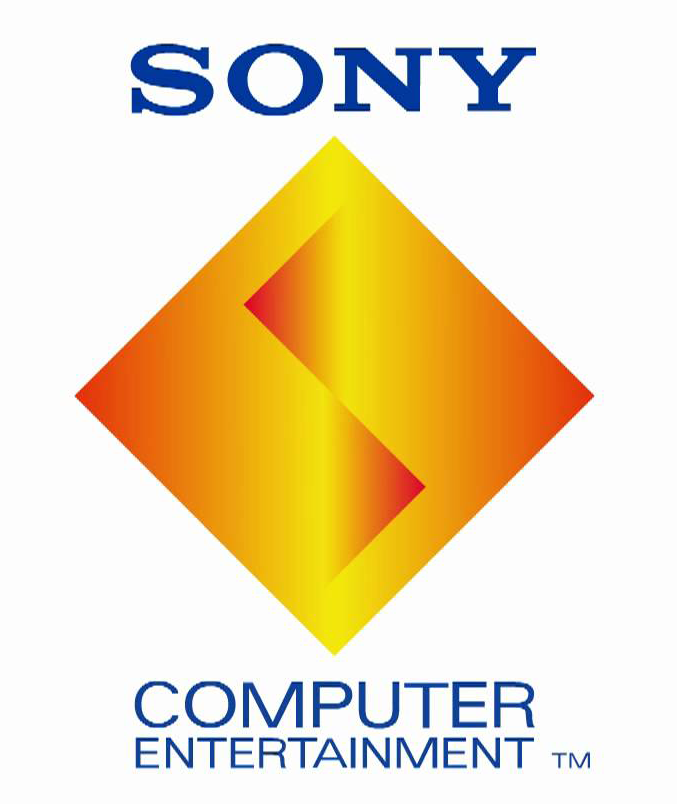
\includegraphics[scale=0.3]{images/SonyMainTarget.png}}
  \caption{Representative picture of Sony, point ARMeet to this image to
    see the different sales on each platform.}
  \label{fig:SonyImage}
\end{figure}

%% Sony
%% Platforms: 6

%% Platform: PS 
%% Games: 1197
%% Total Sales: 730.6812, by country US: 336.5195 EU: 213.6097 JP: 139.82 Other: 40.90947

%% Platform: PS2 
%% Games: 2161
%% Total Sales: 1255.649, by country US: 583.8428 EU: 339.2891 JP: 139.1999 Other: 193.4392

%% Platform: PSP 
%% Games: 1209
%% Total Sales: 294.2983, by country US: 109.1699 EU: 66.67997 JP: 76.77973 Other: 41.4197

%% Platform: PS3 
%% Games: 1331
%% Total Sales: 939.4323, by country US: 393.4895 EU: 330.2896 JP: 80.1898 Other: 135.6793

%% Platform: PS_VITA 
%% Games: 432
%% Total Sales: 54.11987, by country US: 12.58001 EU: 13.12002 JP: 21.93007 Other: 6.460013

%% Platform: PS4 
%% Games: 393
%% Total Sales: 314.2296, by country US: 108.7399 EU: 141.09 JP: 16.00002 Other: 48.34989
